\documentclass[fullscreen=true, bookmarks=true, hyperref={pdfencoding=unicode}]{beamer}
\usepackage[utf8]{inputenc}                                % Кодировка
\usepackage[english,russian]{babel}                        % Переносы
\usepackage{xcolor}                                        % Работа с цветом
\usepackage{amsmath,amssymb,amsfonts}                      % Символы АМО
\usepackage{graphicx}                                      % Графика
\usepackage[labelsep=period]{caption}                      % Разделитель в подписях к рисункам и таблицам
\usepackage{hhline}                                        % Для верстки линий в таблицах
\usepackage{tikz}                                          % Для простых рисунков в документе
\usepackage{fancybox}                                      % Пакет для отрисовки рамок
\usepackage{verbatim}                                      % Для вставки кода в презентацию
\usepackage{animate}                                       % Для вставки видео в презентацию
\usepackage{xmpmulti}                                      % Для вставки gif в презентацию
\usepackage{multirow}

\usetikzlibrary{arrows,snakes,backgrounds}                 % Для отрисовки стрелок

\graphicspath{{images/}}                                   % Путь до рисунков
\setbeamertemplate{caption}[numbered]                      % Включение нумерации рисунков

\definecolor{links}{HTML}{2A1B81}                          % blue for url links
\hypersetup{colorlinks,linkcolor=,urlcolor=links}          % nothing for others

\usetheme{Boadilla}
\usecolortheme{whale}

\usepackage{minted}

\title{Lecture 5. Neural networks intro, backpropagation method}
\author{Alex Avdyushenko}
\institute{Kazakh-British Technical University}
\date{October 8, 2022}
\titlegraphic{
\includegraphics[keepaspectratio,width=0.4\textwidth]{logo_kbtu.png}}

\begin{document}
%\unitlength=2mm

% выводим заглавие
\begin{frame}
\transdissolve[duration=0.2]
\titlepage
\end{frame}

\begin{frame}
  \frametitle{Five-minute questions}
  \begin{itemize}
    \item What is the name of the course?
    \item What is the teacher's name?
    \item What color is the textbook?
  \end{itemize}
\end{frame}

\begin{frame}{To make long story short}
\begin{columns}
    \small
    \begin{column}{.15\paperwidth}
      \onslide <2->
      
\includegraphics[keepaspectratio,       width=.15\paperwidth]{mmf.png}
      2009, master of math
      
      \onslide <1->
      
\includegraphics[keepaspectratio,       width=.15\paperwidth]{pms.png}
      2003, silver medal      
    \end{column}
    \begin{column}{.15\paperwidth}
      \vspace{3cm}
      \onslide <3->
      
\includegraphics[keepaspectratio,       width=.15\paperwidth]{ict.png}
      2014, phd
    \end{column}
    \begin{column}{.15\paperwidth}
      \vspace{1.5cm}
      \onslide <4->
      
\includegraphics[keepaspectratio,       width=.15\paperwidth]{shad.png}
      2016, YDS
    \end{column}
    \begin{column}{.15\paperwidth}
      \onslide <5->
      
\includegraphics[keepaspectratio,       width=.15\paperwidth]{yandex.jpg}
      2015-2018, analyst
    \end{column}
    \begin{column}{.15\paperwidth}
      \onslide <6->
      
\includegraphics[keepaspectratio,       width=.15\paperwidth]{csc.png}
      2016-2022, ed manager
      \vspace{3cm}
    \end{column}
    \begin{column}{.15\paperwidth}
      \onslide <9->
      
\includegraphics[keepaspectratio,       width=.12\paperwidth]{kbtu.png}
      2022+, instructor

      \onslide <8->
      
\includegraphics[keepaspectratio,       width=.12\paperwidth]{yandex.jpg}
      2022+, head of ML ed

      \onslide <7->
      
\includegraphics[keepaspectratio,       width=.12\paperwidth]{spbu.png}
      2019+, docent
    \end{column}
\end{columns}
    
\end{frame}


\begin{frame}
  \frametitle{Tasks solved by neural networks}

  \begin{columns}
      \begin{column}{.3\paperwidth}
      \onslide <1->
      Images: 25\% $\to$ 3.5\% VS 5\% errors by human
      
\includegraphics[keepaspectratio,       width=.3\paperwidth]{image_net.jpg}
      
      \vspace{0.5cm}
      \onslide <4->
      Game Go, 2016
      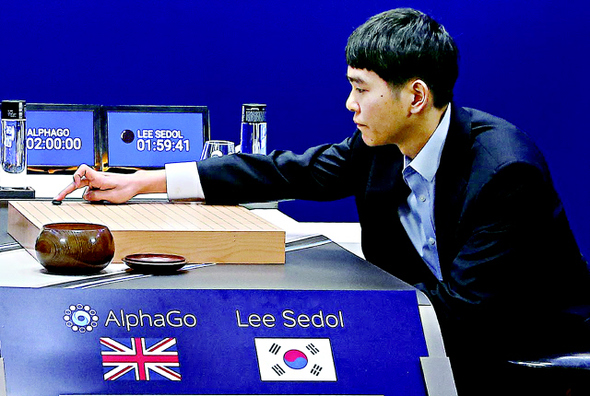
\includegraphics[keepaspectratio,       width=.3\paperwidth]{alpha_go.jpg}
      \end{column}
      
      \begin{column}{.3\paperwidth}
      \onslide <2->
      Texts
      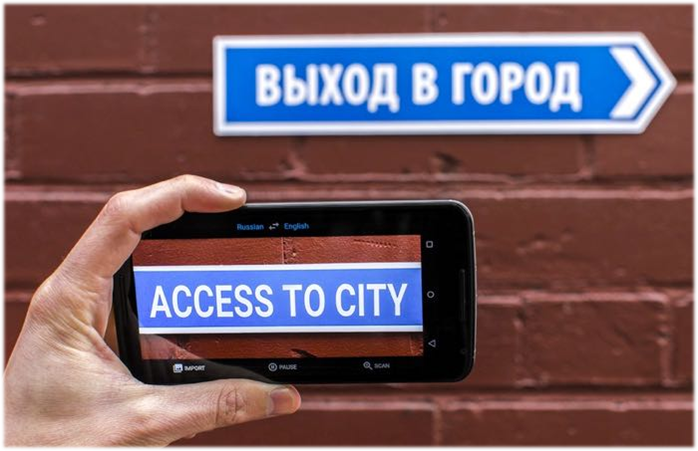
\includegraphics[keepaspectratio,       width=.3\paperwidth]{machine_translation.png}
      
      \vspace{0.4cm}
      \onslide <5->
      StarCraft, 2019
      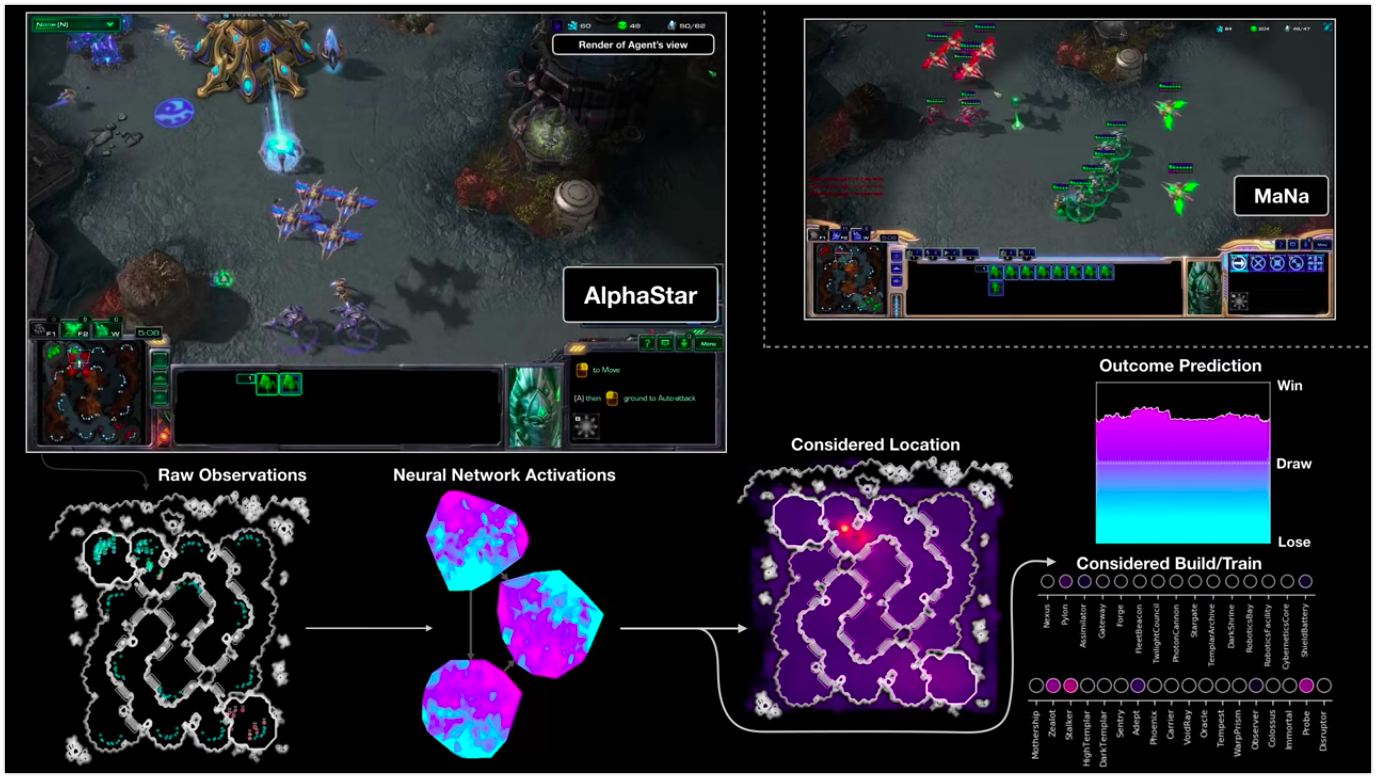
\includegraphics[keepaspectratio,       width=.3\paperwidth]{starcraft.png}
      \end{column}
      
      \begin{column}{.3\paperwidth}
      \onslide <3->
      Voice
      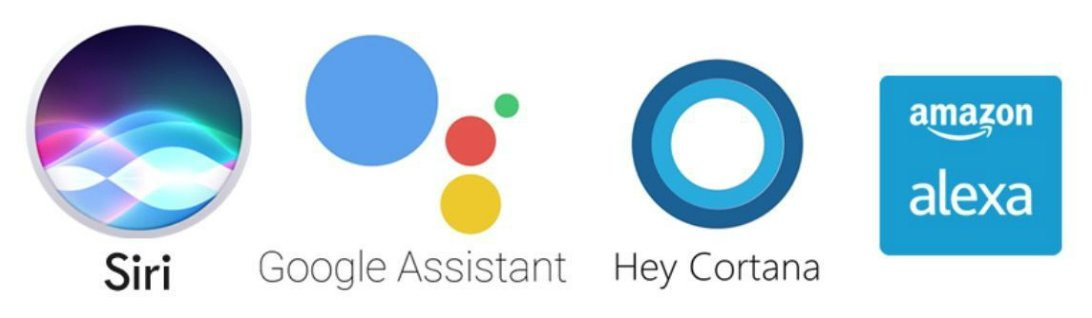
\includegraphics[keepaspectratio,       width=.3\paperwidth]{voice.jpg}
      
      \vspace{0.3cm}
      \onslide <6->
      Protein structure, 2022
      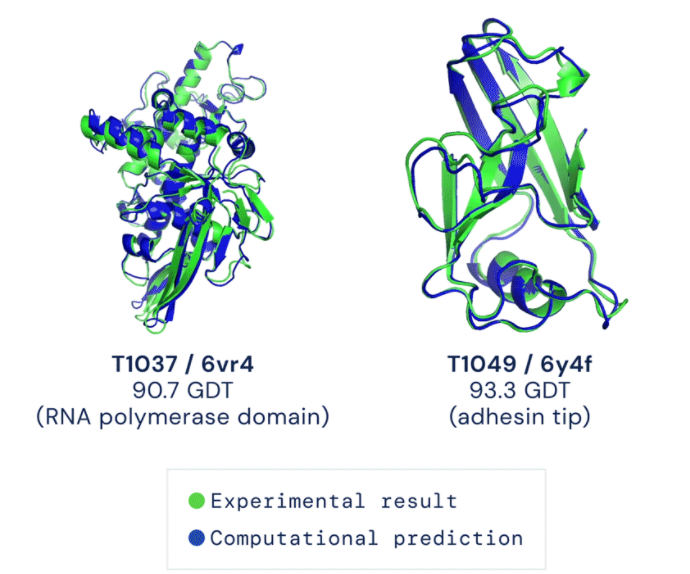
\includegraphics[keepaspectratio,       width=.3\paperwidth]{AlphaFold.png}
      \end{column}
  \end{columns}

\end{frame}


{ % all template changes are local to this group.
    \setbeamertemplate{navigation symbols}{}
    \begin{frame}<article:0>[plain]
        \begin{tikzpicture}[remember picture,overlay]
            \node[at=(current page.center)] {
                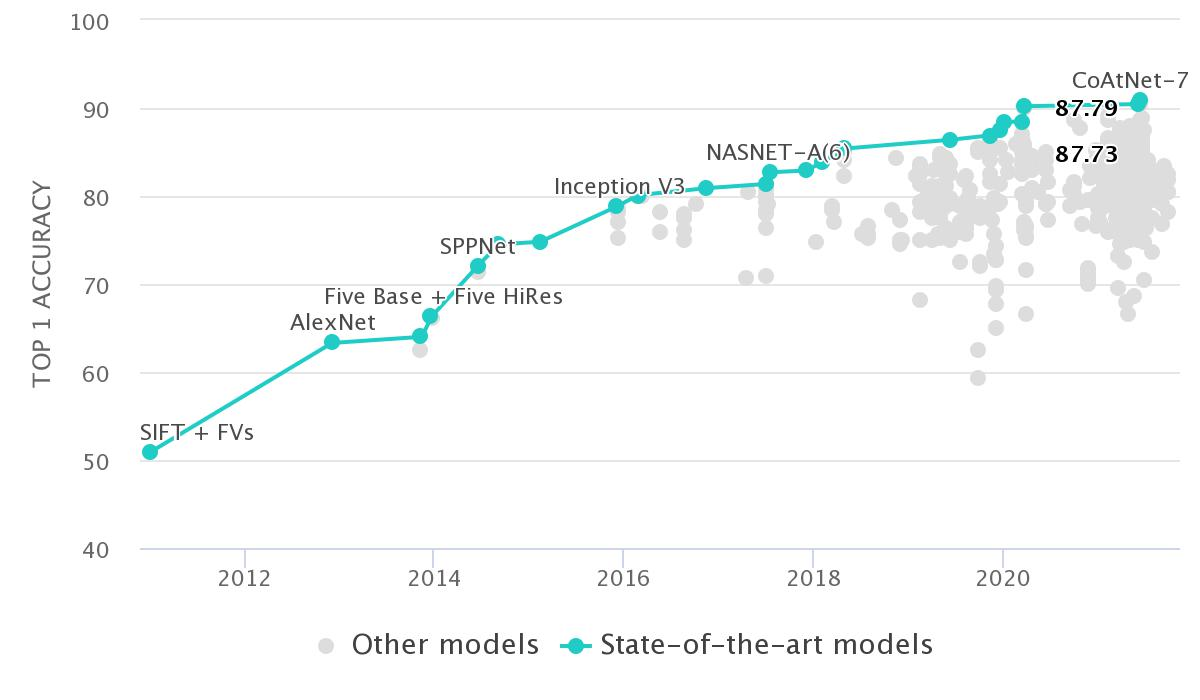
\includegraphics[keepaspectratio,
                                 width=\paperwidth, height=\paperheight]{imagenet_progress_pwc.jpeg}
            };
        \end{tikzpicture}
        
        \vspace{8cm}
        \href{https://paperswithcode.com/sota/image-classification-on-imagenet}{https://paperswithcode.com/sota/image-classification-on-imagenet}
     \end{frame}
}


\begin{frame}
  \frametitle{Linear model}
  \framesubtitle{recall}

 $x^1, x^2, \dots, x^n \in \mathbb{R}$ — numerical features of one object $x$
 
 $w_0, w_1, \dots, w_n \in \mathbb{R}$ — weights of features
 
 $$a(x, w) = \sigma(\left<w, x\right>) = \sigma \left(\sum\limits_{j=1}^n w_j f_j(x) - w_0 \right),$$
 
 $\sigma(z)$ — activation function, for example one of the:
 $\text{sign}(z),\ \frac{1}{1+e^{-z}},\ (z)_+$

\begin{center}
  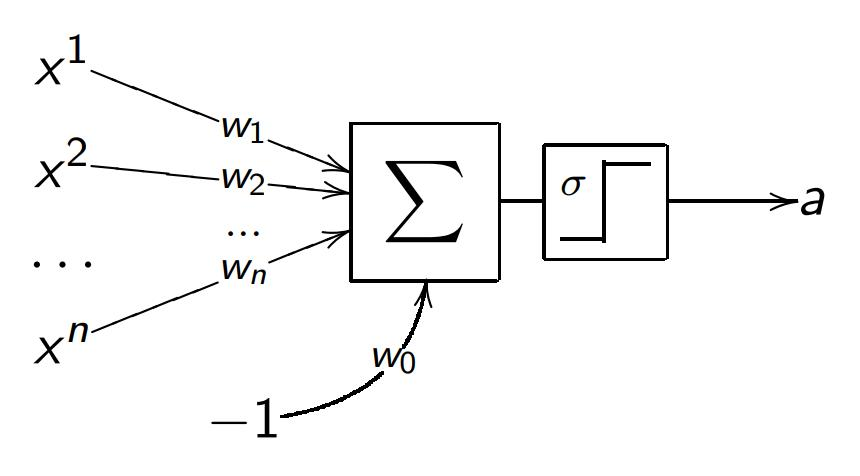
\includegraphics[keepaspectratio, width=.5\paperwidth]{lin_as_nn.jpg}
\end{center}
\end{frame}

\begin{frame}{Neural network as combination of linear models}
\begin{center}
  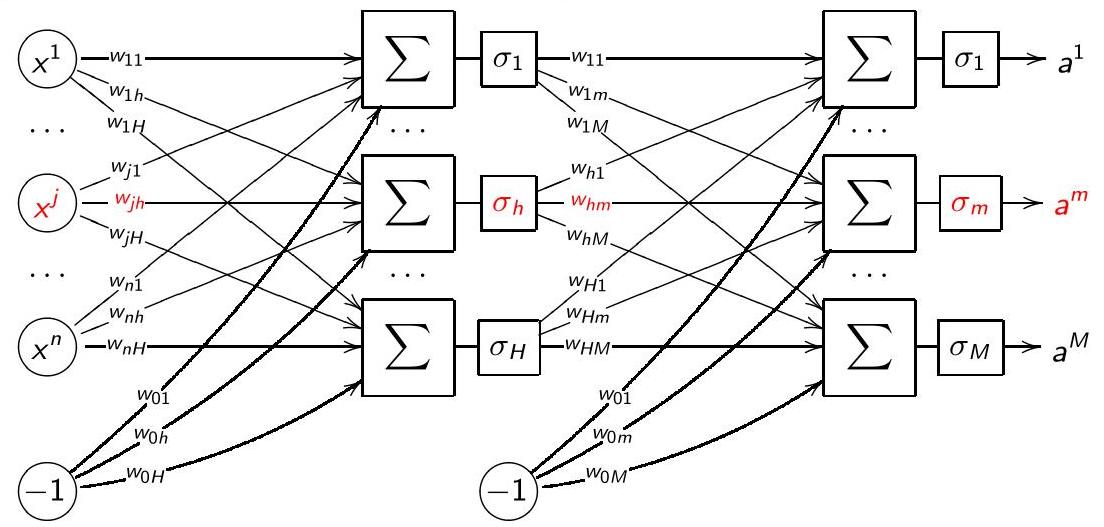
\includegraphics[keepaspectratio, width=.9\paperwidth]{nn_two_layers_cropped.jpg}
\end{center}
\end{frame}


\begin{frame}
  \frametitle{Neural implementation of logic functions}

 Functions AND, OR, NOT from binary variables $x^1$ and $x^2$:
 \begin{center}
 $x^1 \wedge x^2 = [x^1 + x^2 - \frac{3}{2} > 0]$

 $x^1 \vee x^2 = [x^1 + x^2 - \frac{1}{2} > 0]$

 $\neg x^1 = [-x^1 + \frac{1}{2} > 0]$
 \end{center}

\begin{center}
  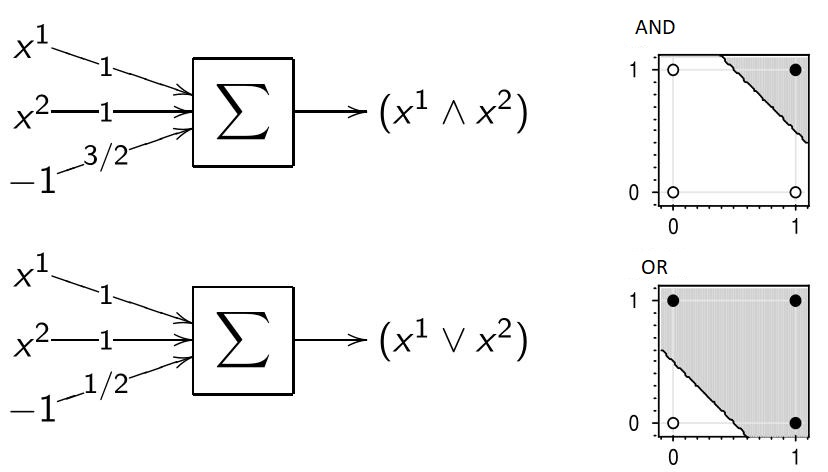
\includegraphics[keepaspectratio, width=.6\paperwidth]{and_or.jpg}
\end{center}

\end{frame}


\begin{frame}
  \frametitle{Logic function XOR}
  Function $x^1 \bigoplus x^2 = [x^1 \neq x^2]$ 

  {\bf Is not implementable} by one neuron
  
  There are two ways to implement:
  \begin{itemize}
      \item By adding a non-linear feature
      $x^1 \bigoplus x^2 = [x^1 + x^2 - { \color{red}2x^1 x^2} - \frac12 > 0]$
      \item With a network (two-layer superposition) of AND, OR, NOT functions:
      $x^1 \bigoplus x^2 = [(x^1 \vee x^2) - (x^1 \wedge x^2) - \frac12 > 0]$.
  \end{itemize}

\begin{center}
  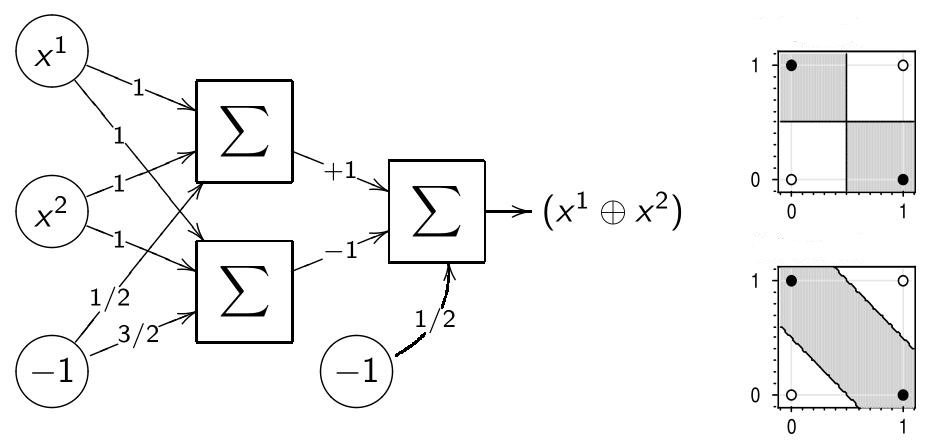
\includegraphics[keepaspectratio, width=.7\paperwidth]{xor_nn.jpg}
\end{center}

\end{frame}


\begin{frame}
  \frametitle{Expressive power of a neural network}
  \begin{itemize}
      \item A two-layer network in $\{0, 1\}^n$ allows us to implement an arbitrary Boolean function
      \pause
      \item A two-layer network in $\mathbb{R}^n$ allows us to separate an arbitrary convex polyhedron
      \pause
      \item A three-layer network in $\mathbb{R}^n$ allows you to separate an arbitrary polyhedral region (may not be convex or even connected)
      \pause
      \item With the help of linear operations and one non-linear activation function $\sigma$ any continuous function can be approximated with any desired accuracy
      \pause
      \item For some special classes of deep neural networks, they have been proven to have exponentially greater expressive power than shallow networks. 

      {\small
      \href{https://arxiv.org/pdf/1711.00811.pdf}{V. Khrulkov, A. Novikov, I. Oseledets. Expressive power of recurrent neural networks, Feb 2018, ICLR}}
  \end{itemize}
\end{frame}


\begin{frame}
  \frametitle{ImageNet}
  Annotated Image Dataset Project
  \begin{itemize}
      \item 14M+ images
      \item 20K+ classes
  \end{itemize}

  \begin{center}
  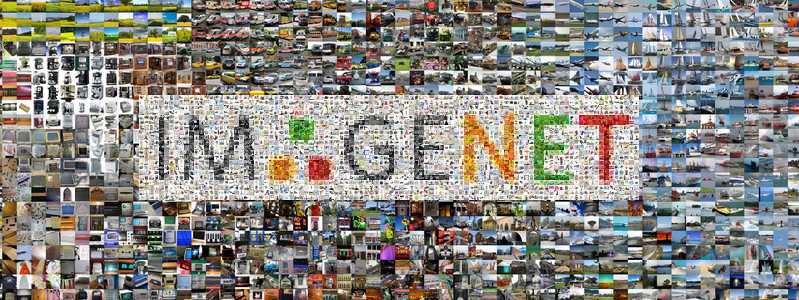
\includegraphics[keepaspectratio, width=0.9\paperwidth]{ImageNet-Large-Scale.jpg}      
  \end{center}
\end{frame} 


\begin{frame}
  \frametitle{The development of convolutional networks}
  \framesubtitle{Or a brief history of ImageNet}
  \begin{center}
    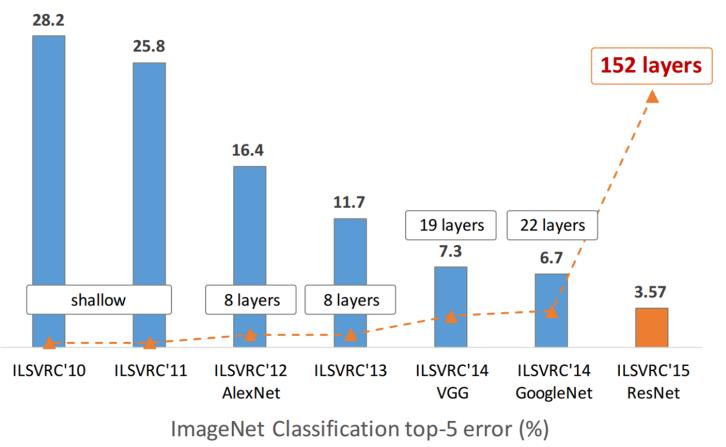
\includegraphics[keepaspectratio, height=0.7\paperheight]{image-net-history.jpg}
  \end{center}
\end{frame}


\begin{frame}
  \frametitle{Two-layer neural network with M-dimensional output}

  \begin{center}
    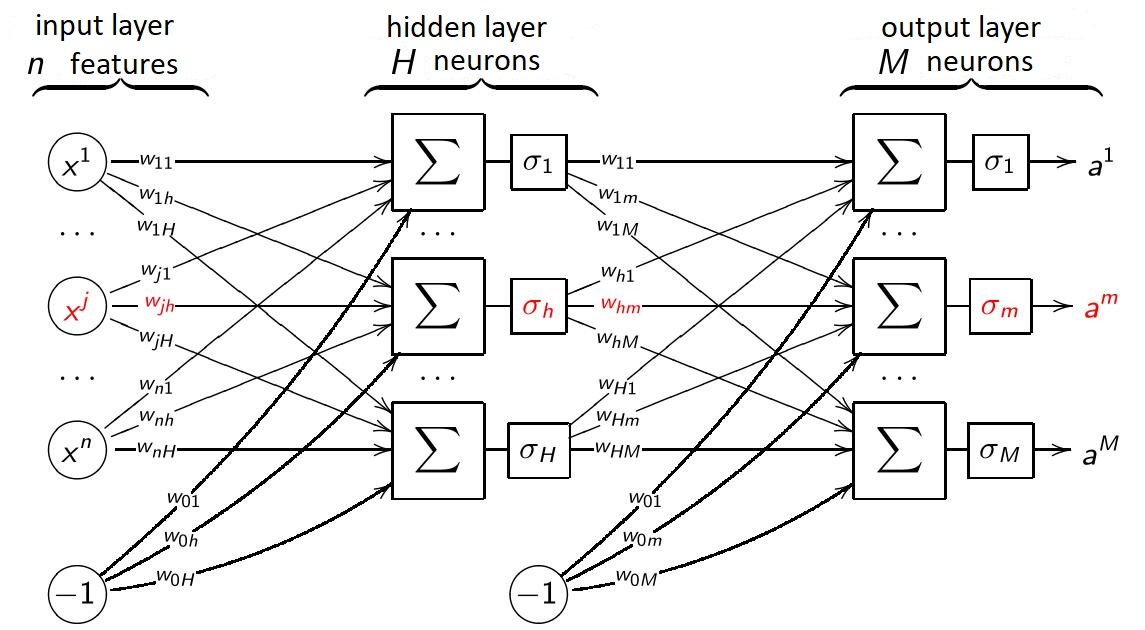
\includegraphics[keepaspectratio,                     height=0.6\paperheight]{nn_two_layers.jpg}
  \end{center}
  
  Model parameter vector $w \equiv (w_{jh}, w_{hm}) \in \mathbb{R}^{Hn + H + MH + M}$
\end{frame}


\begin{frame}
    \begin{block}{Question 1}
    Where do these amounts of parameters come from?
    \end{block}
\end{frame}


\begin{frame}
  \frametitle{MNIST in PyTorch}
  \framesubtitle{Demo}
  
  \href{https://github.com/avalur/ml-course-kbtu/tree/main/week05_nn_backprop/demo_MNIST_in_PyTorch.ipynb}{Notebook at github}

  \vspace{1.5cm}

  Source: \href{https://nextjournal.com/gkoehler/pytorch-mnist}{https://nextjournal.com/gkoehler/pytorch-mnist}
  
\end{frame}


\begin{frame}
  \frametitle{Neural network}

  \begin{center}
    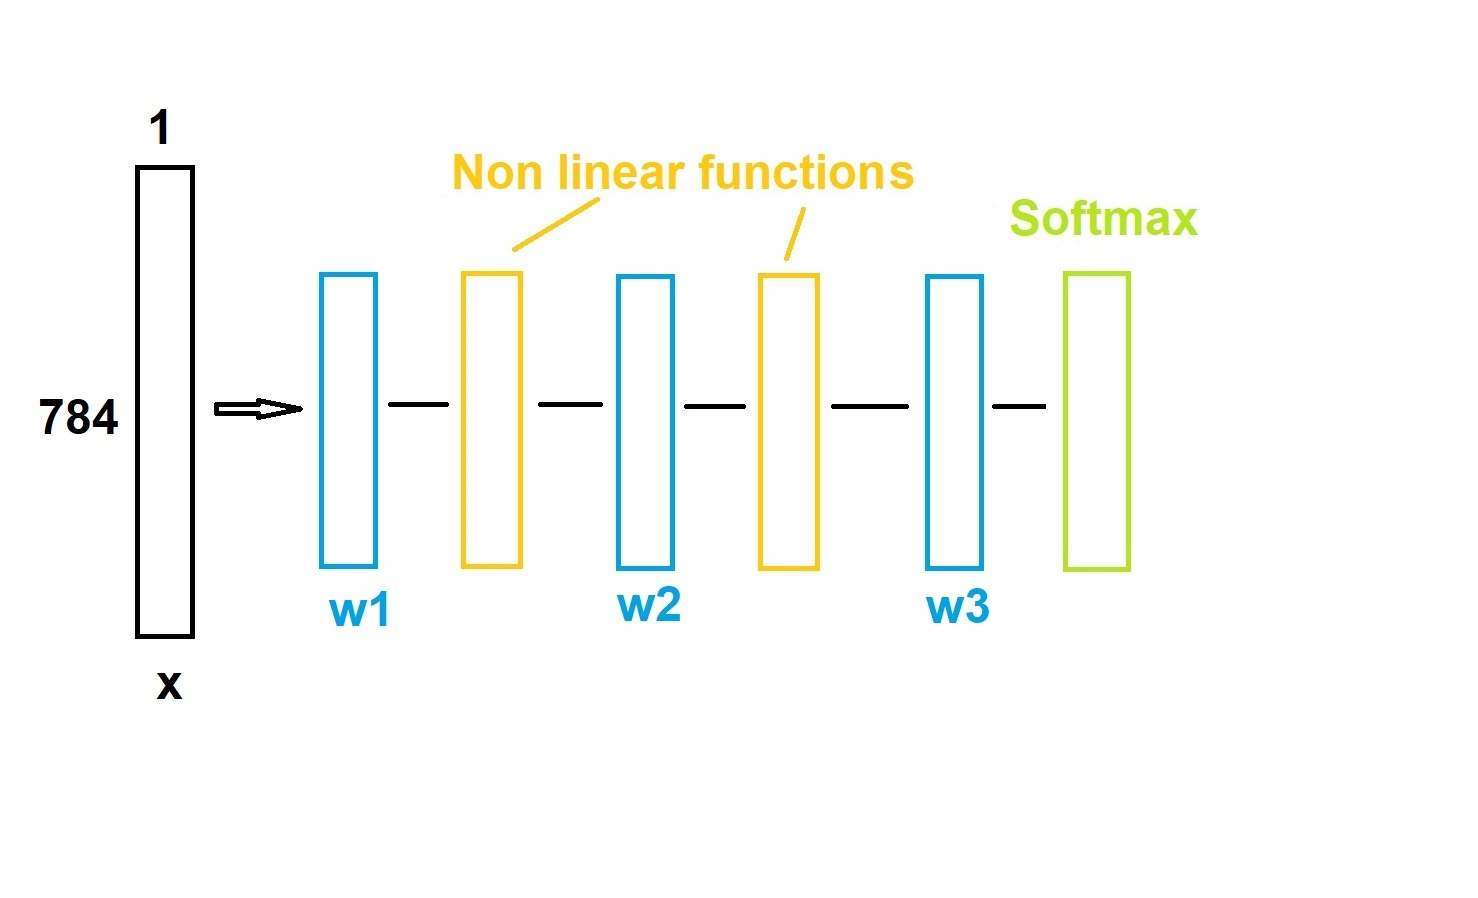
\includegraphics[keepaspectratio, width=\paperwidth]{nn_scheme.jpg}
  \end{center}
\end{frame}


\begin{frame}
\frametitle{Sigmoid Activation Functions}
   \begin{itemize}
     \item Logistic sigmoid
     $\sigma(z) = \frac{1}{1+\exp(-z)}$

     \pause
     \item Hyperbolic tangent
     $\tanh(z) = \frac{\exp(z)-\exp(-z)}{\exp(z)+\exp(-z)}$

     \pause
     \item continuous approximations of threshold function
     
     \pause
     \item can lead to vanishing gradient problem and "paralysis" of the network
   \end{itemize}
\end{frame}

% import matplotlib.pyplot as plt
% import numpy as np

% fig, ax1 = plt.subplots(1, 1)

% ax1.set_xlabel('x')

% x1 = np.linspace(-3.5, 3.5, num=100)
% ax1.set_ylim(-1.1, 2.1)

% sigmoid = 1 / (1 + np.exp(-x1)) 
% ax1.plot(x1, sigmoid, 'r', label='sigmoid')
% tanh = np.tanh(x1) 
% ax1.plot(x1, tanh, 'g--', label='tanh')
% relu = x1 * (x1 > 0) 
% ax1.plot(x1, relu, 'k+', label='relu')
% leaky_relu = x1 * (x1 > 0) + 0.1 * x1 * (x1 < 0) 
% ax1.plot(x1, leaky_relu, 'b-', label='leaky_relu, 0.1')

% step = 1 * (x1 > 0) 
% ax1.plot(x1, step, '-', label='step')

% ax1.grid(True)

% fig.set_size_inches(14, 6)
% plt.legend(loc='best')
% plt.show()

\begin{frame}
  \frametitle{Let's look at the charts}
  \begin{center}
    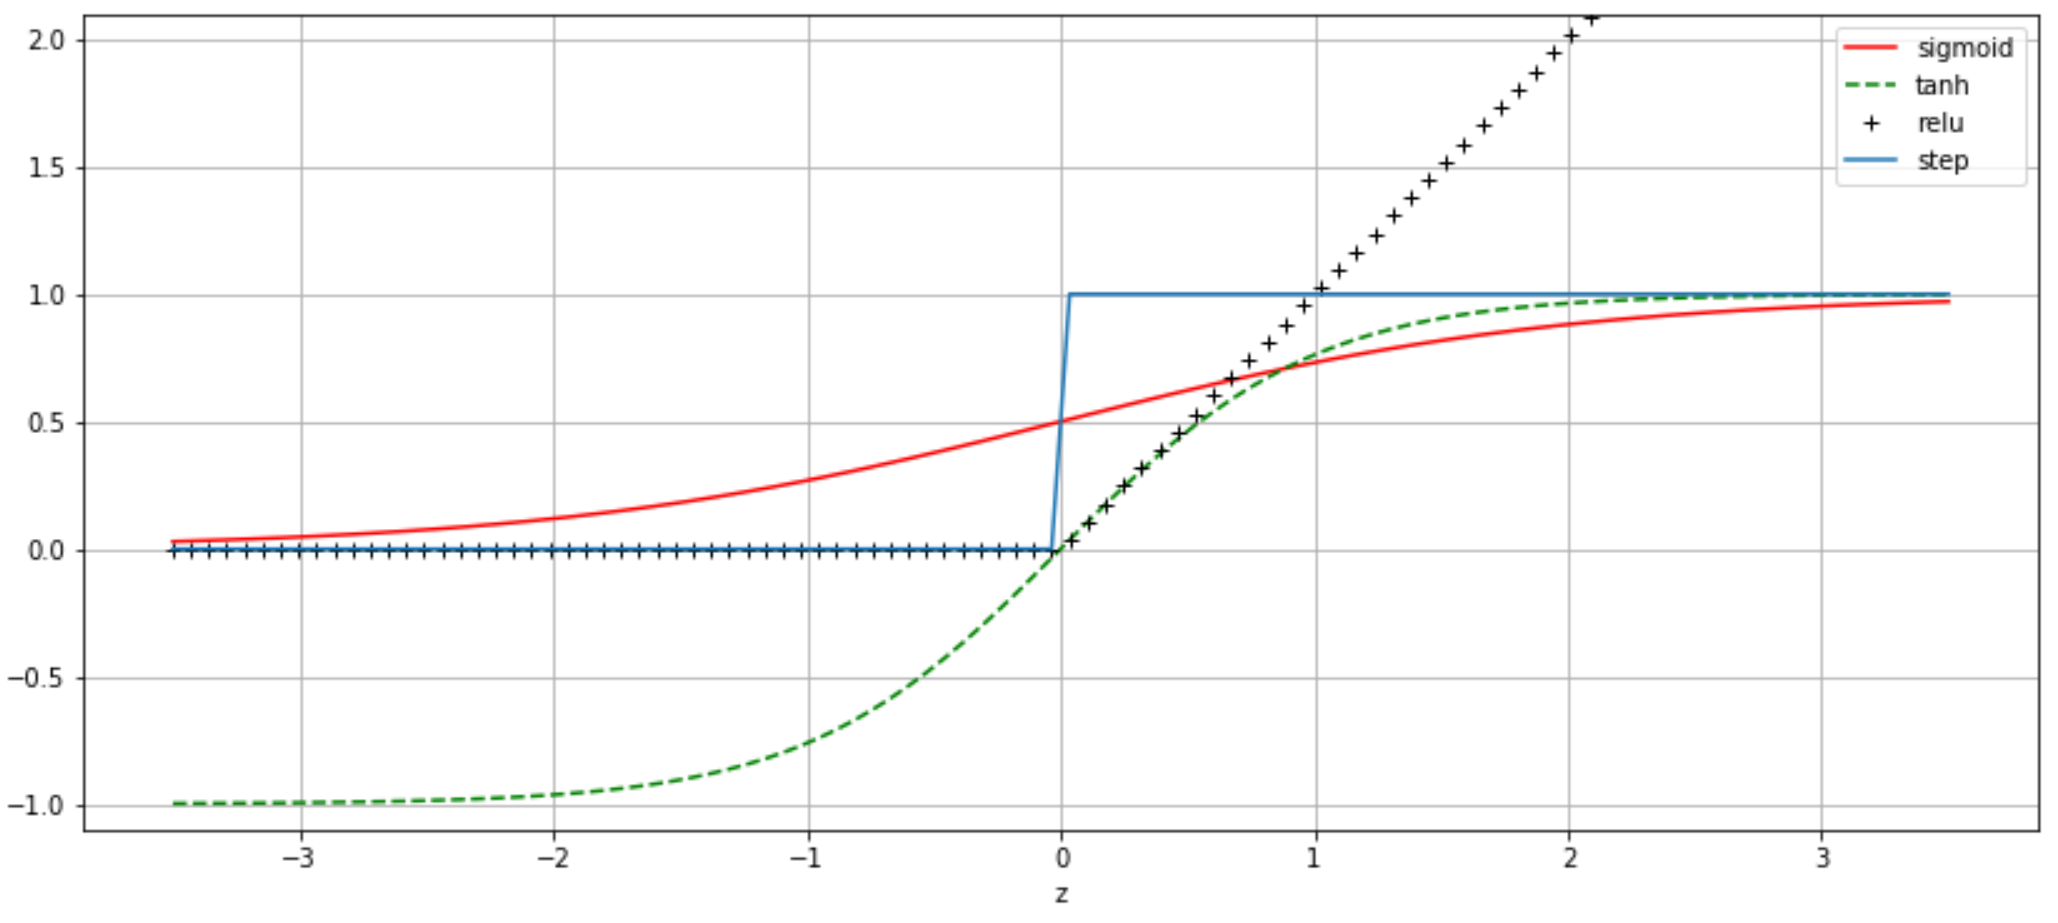
\includegraphics[keepaspectratio, width=0.9\paperwidth]{sigm_relu.png}
  \end{center}
\end{frame}


\begin{frame}
  \frametitle{ReLU — Rectified Linear Unit}
  $$\text{ReLU}(z) = \max(0, z)$$

  Motivation:

  $\sigma(5) \approx 0.9933, \sigma(10) \approx 0.9999$

  $f(x) = \sigma(x + \frac12) + \sigma(x - \frac12) + \sigma(x - \frac32) + \sigma(x - \frac52) + \dots$

  \begin{center}
    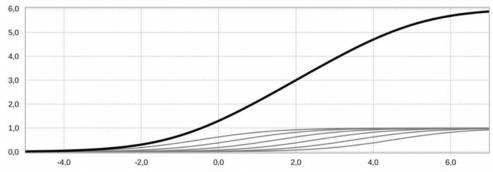
\includegraphics[keepaspectratio, width=0.7\paperwidth]{from_nikolenko.jpg}
  \end{center}

  \noindent\rule{8cm}{0.4pt}

  {\it \small (in Russian) Deep Learning: Dive into The World of Neural Networks, S.I. Nikolenko, A.A. Kadurin, E.O. Arkhangelskaya, Piter, 2017}
\end{frame}


\begin{frame}
  \frametitle{ReLU — Rectified Linear Unit}
  $$\int \sigma(x) dx = \log(1 + e^x) + C$$

  It turns out that $f(x)$ is the Riemannian sum of such an integral:

  $$\int\limits_{1/2}^\infty \sigma(x + \frac12 - y) dy $$

  \begin{multline*}
    f(x) = \sum\limits_{i=0}^\infty \sigma(x + \frac12 - i) \approx \int \limits_{1/2}^\infty \sigma(x + \frac12 - y) dy = \\
    = [-\log(1 + \exp(x+\frac12 - y))]_{y=1/2}^{y=\infty} = \log(1 + \exp(x)) = \text{Softplus}(x)
  \end{multline*}
\end{frame}


\begin{frame}
  \frametitle{Let's look at the charts}
  \begin{center}
    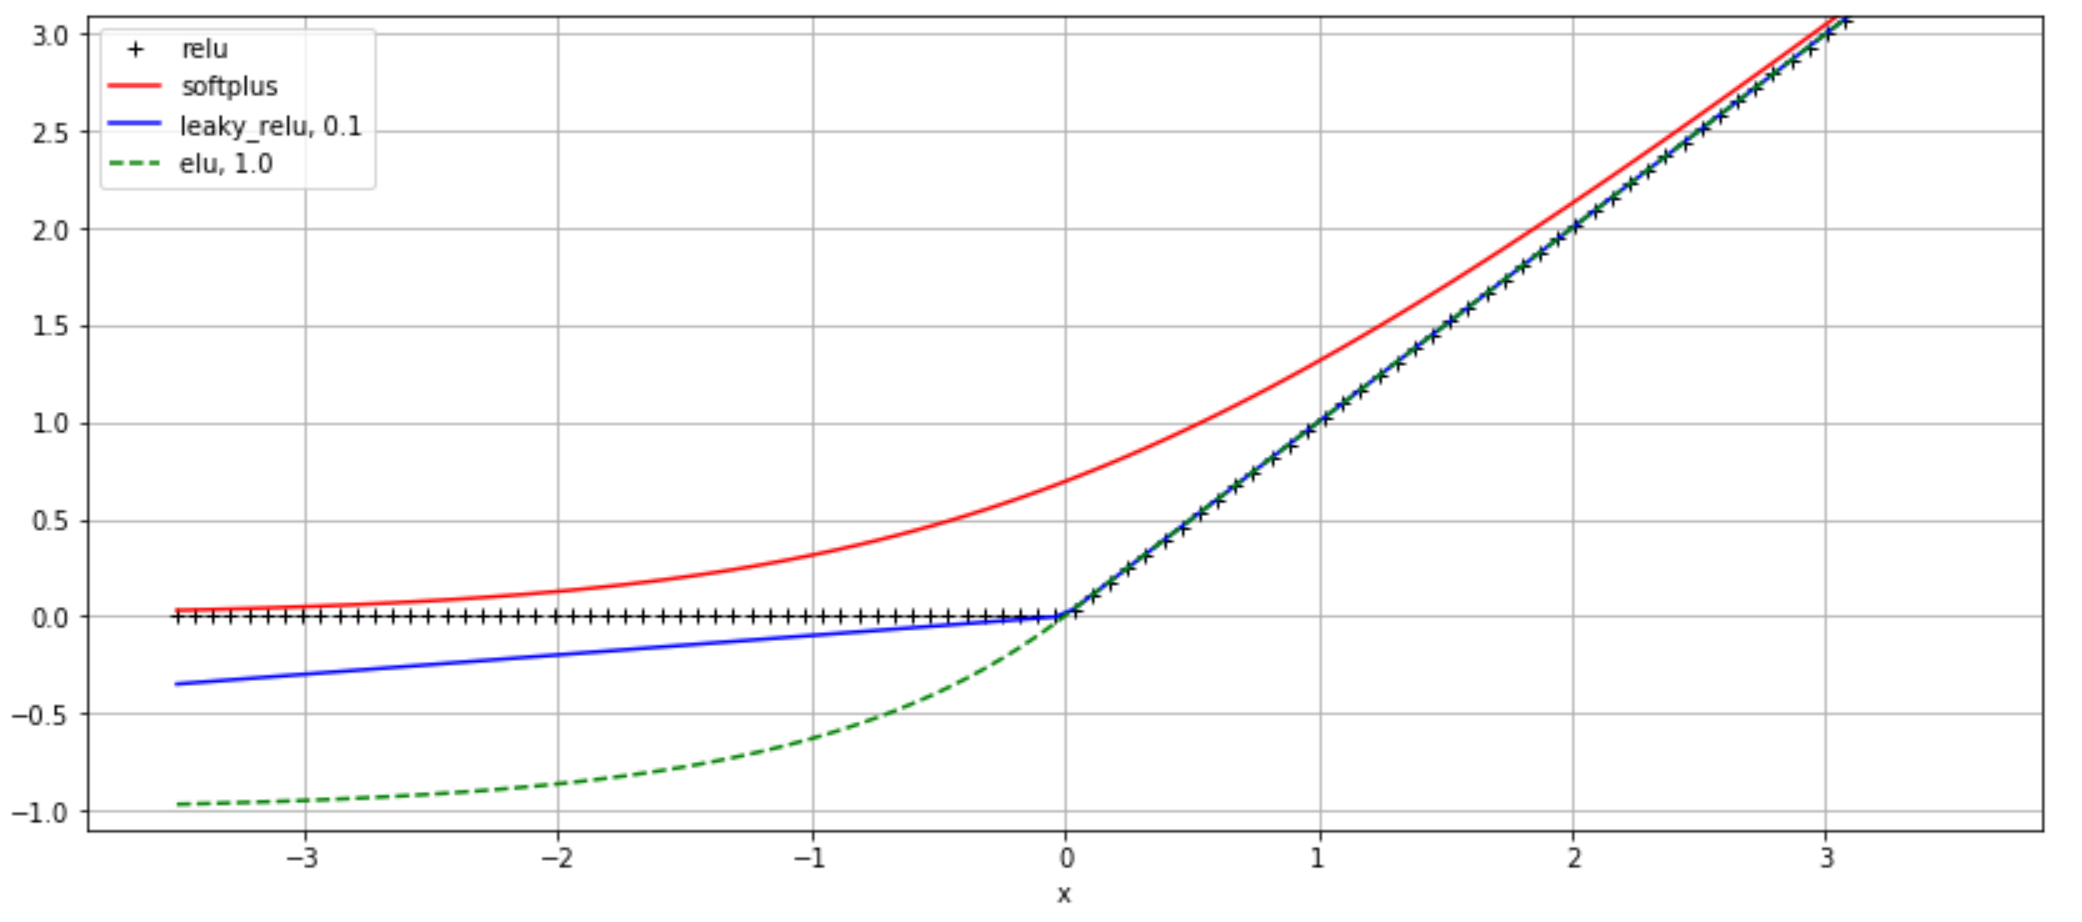
\includegraphics[keepaspectratio, width=0.9\paperwidth]{relu_softplus.png}
  \end{center}
\end{frame}


\begin{frame}{Regularization}

\begin{columns}
  \begin{column}{0.5\paperwidth}
    $$ L(W, b) = - \sum\limits_j \ln \frac{e^{(x_jW + b)_{y_j}}}{\sum\limits_i e^{(x_jW + b)_{i}}} + \lambda R(W, b)$$
    
    $$R(W, b) = \|W\|_2^2 + \|b\|_2^2 $$
      
    $$\|b\|_2^2 = b_0^2 + \dots + b_k^2$$
  \end{column}
  \begin{column}{0.45\paperwidth}
      \begin{center}
        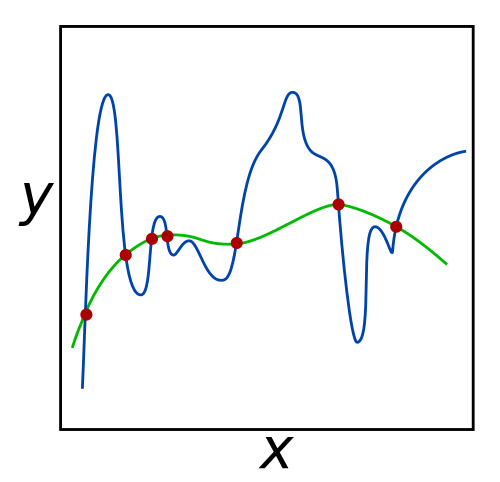
\includegraphics[keepaspectratio, width=0.3\paperwidth]{regularization.png}
      \end{center}    
  \end{column}
\end{columns}
\end{frame}


\begin{frame}{Backpropagation method}
  \framesubtitle{Computational graph}

  Let's include $b$ into $W$

  $$ L(W) = - \sum\limits_j \ln p(c = y_j|x_j) + \lambda R(W) \\ \ $$

      \begin{center}
        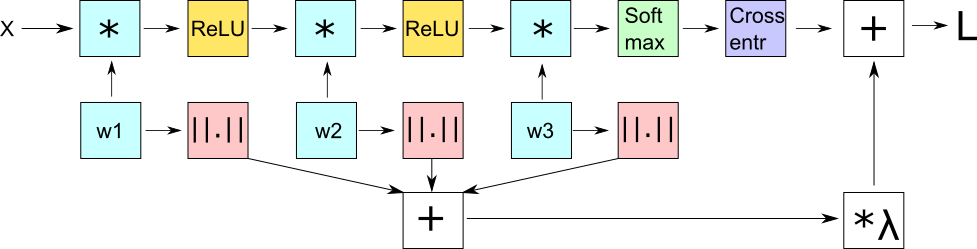
\includegraphics[keepaspectratio, width=0.8\paperwidth]{graph_calc.png}
      \end{center}

We want to find the gradients of the loss function $L$ over all inputs of the computation graph
\end{frame}


\begin{frame}{A simple example}

Derivative of a function composition $f(g(x))\ \ \to \frac{df}{dx} = \frac{df}{dg} \frac{dg}{dx}$

Let $f(x, w) = 1 + e^{w_1x + w_0}$

\begin{center}
  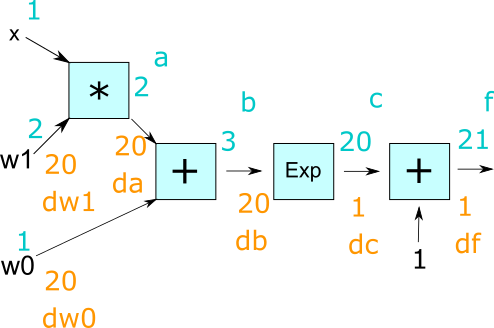
\includegraphics[keepaspectratio, width=0.5\paperwidth]{simple_graph.png}
\end{center}

$$ \frac{\partial f}{\partial f} = 1, \ f = c + 1, \ dc = \frac{\partial f}{\partial c} = 1, \dots$$    
\end{frame}


\begin{frame}{General scheme for calculating the gradient}

\begin{center}
  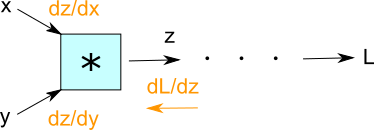
\includegraphics[keepaspectratio, width=0.5\paperwidth]{backprop_scheme.png}
\end{center}
\end{frame}


\begin{frame}{Backpropagation recap}

As a result, we are able to calculate all the gradients with simple operations of the reverse pass through the graph and:

\begin{itemize}
    \pause
    \item we did not write out the entire derivative analytically
    \pause
    \item at each step a simple function is differentiated
    \pause
    \item we need only one pass along the calculation graph
    \pause
    \item parallelization is possible
\end{itemize}

\end{frame}


\begin{frame}
  \frametitle{Summary}
  \begin{itemize}
      \pause
      \item Neuron = linear classificator or regressor
      \pause
      \item Neural network = superposition of neurons with non-linear activation functions
      \pause
      \item Backpropagation = fast differentiation of superpositions. Allows you to train networks of almost any configuration
      \pause
      \item Methods for improving convergence and quality:
      \begin{itemize}
          \item training on mini-batches
          \item various activation functions
          \item regularization
      \end{itemize}
      \pause
      \item Was not at this lecture — will be in the next lectures of the course:
      \begin{itemize}
          \item various optimization algorithms: adam, RMSProp
          \item dropout
          \item choice of initial approximation and its connection with activation functions
      \end{itemize}
  \end{itemize}
\end{frame}


\begin{frame}{What else can you watch?}
  \begin{itemize}
      \pause
      \item In Stanford's course: \href{http://cs231n.github.io/optimization-2/}{http://cs231n.github.io/optimization-2/}
      \pause
      \item 3blue1brown about backprop: \href{https://www.youtube.com/watch?v=Ilg3gGewQ5U}{https://www.youtube.com/watch?v=Ilg3gGewQ5U}
      \pause
      \item The third lecture of the course "Deep Learning on the fingers" from Semyon Kozlov (in Russian): \href{https://www.youtube.com/watch?v=kWTC1NvL894}{https://www.youtube.com/watch?v=kWTC1NvL894}
  \end{itemize}
\end{frame}


\begin{frame}{In the case of a two-layer neural network}

Output values of the network $a^m(x_i), m = 1 \dots M$ on the object $x_i$:

$$a^m(x_i) = \sigma_m \left( \sum\limits_{h=0}^H w_{hm} {\color{red}u^h(x_i)} \right)$$

$${\color{red}u^h(x_i)} = \sigma_h \left( \sum\limits_{j=0}^J w_{jh} f_j(x_i) \right)$$

Let for definiteness

$$\mathcal{L}_i (w) = \frac12 \sum\limits_{m=1}^M (a^m(x_i) - y_i^m)^2$$

{\bf Intermediate task}: Partial Derivatives
$\frac{\partial \mathcal{L}_i(w)}{\partial a^m},\ \ \frac{\partial \mathcal{L}_i(w)}{\partial u^h}$    
\end{frame}


\begin{frame}{Fast differentiation. Auxiliary gradients}

{\bf Intermediate task}: Partial Derivatives

$$\frac{\partial \mathcal{L}_i(w)}{\partial a^m} = a^m(x_i) - y_i^m = \varepsilon_i^m$$

is the error at the output layer (for quadratic losses);

$$\frac{\partial \mathcal{L}_i(w)}{\partial u^h} = \sum\limits_{m=1}^M (a^m(x_i) - y_i^m) \sigma_m^ \prime w_{hm} =
  \sum\limits_{m=1}^M \varepsilon_i^m \sigma_m^\prime w_{hm} = \varepsilon_i^h$$

— let's call it {\it an error on a hidden layer}.

It turns out that $\varepsilon_i^h$ is calculated from $\varepsilon_i^m$ if the network is run backwards:

\begin{center}
  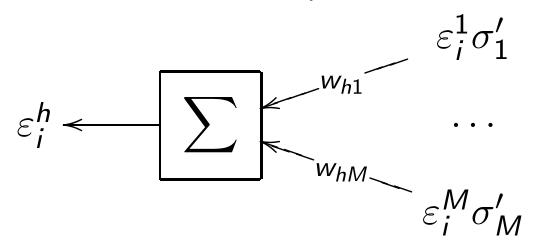
\includegraphics[keepaspectratio, width=0.45\paperwidth]{backprop_eps.jpg}
\end{center}
\end{frame}


\begin{frame}{Fast gradient calculation}

Now, given the partial derivatives of $\mathcal{L}_i(w)$ with respect to $a^m$ and $u^h$, it is easy to write out the gradient of $\mathcal{L}_i(w)$ with respect to the weights of $w$:

$$\frac{\partial \mathcal{L}_i(w)}{\partial w_{hm}} = \frac{\partial \mathcal{L}_i(w)}{\partial a^m} \frac{ \partial a^m}{\partial w_{hm}} = \varepsilon_i^m \sigma^\prime_m u^h(x_i),$$

$m = 1, \dots, M, h = 0, \dots, H$

$$\frac{\partial \mathcal{L}_i(w)}{\partial w_{jh}} = \frac{\partial \mathcal{L}_i(w)}{\partial u^h} \frac{ \partial u^h}{\partial w_{jh}} = \varepsilon_i^h \sigma^\prime_h f_j(x_i),$$ 

$h = 1, \dots, H, j = 0, \dots, n$
\end{frame}


\begin{frame}{Backpropagation algorithm}

\begin{enumerate}
    \item initialize weights $w_{jh}, w_{hm}$
    
    {\bf repeat}
    \item select object $x_i$ from $X^\ell$ (e.g. randomly)
    \item forward pass
    
      $u_i^h = \sigma_h \left(\sum_{j=0}^J w_{jh}x_i^j \right), h = 1, \dots, H$
    
      $a_i^m = \sigma_m \left(\sum_{h=0}^H w_{hm}u_i^h \right), \varepsilon_i^m = a_i^m - y_i^m, m = 1, \dots, M$
    
      $\mathcal{L}_i = \sum_{m=1}^M (\varepsilon_i^m)^2$

    \item backward
    
      $\varepsilon_i^h =\sum\limits_{m=1}^M \varepsilon_i^m \sigma_m^\prime w_{hm}, h = 1\dots H$

    \item gradient step
    
      $w_{hm} = w_{hm} - \eta \varepsilon_i^m\sigma_m^\prime u_i^h, h = 0, \dots, H, m = 1\dots M$

      $w_{jh} = w_{jh} - \eta \varepsilon_i^h\sigma_h^\prime x_i^j, j = 0, \dots, n, h = 1\dots H$

    \item $Q = (1 - \lambda)Q + \lambda \mathcal{L}_i$

    {\bf until} Q stabilizes    
\end{enumerate}
\end{frame}


\begin{frame}
  \frametitle{Expressive power of a neural network}

   $\sigma(z)$ is a sigmoid function if $\lim\limits_{z \to -\infty} \sigma(z) = 0$ and $\lim\limits_{z \to +\infty} \sigma( z) = 1$
   
   \begin{block}{Cybenko's theorem}
   (based on Kolmogorov's theorem on the representability of multidimensional functions)

   If $\sigma(z)$ is a continuous sigmoid, then for any function $f(x)$ continuous on $[0,1]^n$ there are values of the parameters $w_h \in \mathbb{R}^n,\ w_0 \in \mathbb{R},\ \alpha_h \in \mathbb{R}$ that is a one-layer network

   $$a(x) = \sum\limits_{h=1}^H \alpha_h \sigma(\left<x, w_h\right> - w_0)$$

   approximates $f(x)$ uniformly with any accuracy $\varepsilon$:

   $|a(x) - f(x)| < \varepsilon$, for all $x \in [0, 1]^n$
   \end{block}
  
  {\tiny \it G. Cybenko. Approximation by Superpositions of a Sigmoidal Function. Mathematics of Control, Signals, and Systems (MCSS) 2 (4): 303--314 (Dec 1, 1989)}
\end{frame}

\end{document}